\documentclass{llncs2e/llncs}
%
\usepackage{makeidx}  % allows for indexgeneration
\usepackage{graphicx}
\usepackage{color}
\usepackage{amssymb}
\usepackage{amsmath}
\usepackage{listings}
\usepackage{subcaption}
\captionsetup{compatibility=false}
%
\begin{document}
%
\pagestyle{headings}  % switches on printing of running heads
%
\title{Implementing a C Memory Model Supporting Integer-Pointer Casts in CompCert}
%
\titlerunning{Integer-Pointer Casts Semantics in CompCert}  % abbreviated title (for running head)
\author{Aur\`ele Barri\`ere}
%
\authorrunning{Aur\`ele Barri\`ere} % abbreviated author list (for running head)
%
\institute{\'Ecole Normale Sup\'erieure de Rennes, France\\
\email{aurele.barriere@ens-rennes.fr}\\ 
}

\maketitle              % typeset the title of the contribution

\hrulefill

\begin{center}
  \textbf{Supervisor: } Professor Chung-Kil Hur\\
  Seoul National University, South Korea
\end{center}

\hrulefill

\begin{center}
  \textbf{May 15 2017 - August 4 2017}
\end{center}

\vfill
\begin{center}

\includegraphics[width=4cm]{img/enslogo.png}
\quad\quad\quad

\includegraphics[width=4cm]{img/snulogo.png}
\end{center}
\vfill
\begin{abstract}
  The ISO C standard does not define semantics for integer-pointer casts. The certified C compiler CompCert uses an abstract memory model which allows for many optimizations, but in which the behavior of such casts is undefined. In~\cite{DBLP:conf/pldi/KangHMGZV15}, Kang et al. present a formal memory model that supports integer-pointer casts semantics, while still allowing common optimizations.
  We show the relevance of this model by implementing both the memory model and the cast semantics in CompCert. We present the changes that need to be done, both in the way CompCert transforms C programs and in the proofs.
\keywords{CompCert, C Memory Model, Integer-Pointer Cast, Optimization}
\end{abstract}
%
\newpage

\def\todo#1{{\color{red}TODO:\quad#1}}
\def\addref#1{{\color{red}$[$#1$]$}}
\def\undef{\textit{undef}}

\section{Introduction}
When compiling critical software written in C, one expects from the compiler to not introduce any bugs, or any behavior that wasn't specified in the C source code.
% compcert and coq
To meet this expectation, CompCert~\cite{DBLP:journals/cacm/Leroy09} is a formally verified C compiler.
It uses the Coq Proof Assistant~\cite{coq} to prove that the compiled code and the source code have the same observable behavior, as defined by the ISO C Standard~\cite{iso}.
CompCert also aims to provide performance of the generated code, and implements several common optimizations. Compiled code runs approximately 10\% slower than code compiled with \texttt{GCC4 -O1}~\cite{compcertwebsite}.
As of today, CompCert is a trusted compiler; despite many efforts~\cite{DBLP:conf/pldi/YangCER11}, no bug have been discovered within the verified parts of CompCert.
CompCert currently supports all of the ISO C 99 Standard, with very few exceptions~\cite{compcertwebsite}.

% iso c and semantics
However, the ISO C standard itself does not define semantics for every syntactically valid C program.
Many C programs are said to have \textit{unspecified behavior} or \textit{undefined behavior}, meaning that conforming compilers can produce any compiled code.
Despite the lack of semantics, many C programmers are using such programs and expect a precise result. %not a very good sentence
This leads to difficult bugs~\cite{DBLP:conf/apsys/WangCCJZK12} and the impossibility of proving that the compiled code behaves as expected.

% integer pointer casts
One popular unspecified feature of the C language is the casting between integer and pointer values.
Such casts have many uses in real C programs. For instance, pointer to integer cast is used in the Linux Kernel or JVM implementations for bit-wise operations on pointers. Integer arithmetic on pointers is used in Linux, FreeBSD, QEMU and others~\cite{cerberus}. Another common usage is to use the bit representation of a pointer as an indexing key of a hash table (used for instance in the C++ standard library).
When compiled with most compilers, those programs behave as expected from the programmers. But these intuitive semantics have not been formalized in the C standard.

% motivation of the Kanget al. paper
Defining a precise, formal semantics for integer-pointer casting and pointer manipulation would allow CompCert to compile even more C programs in a certified way.
The semantics of pointer manipulation depends on the memory model of the compiler.
As of today, CompCert uses a logical memory model~\cite{leroy:hal-00703441}, where every memory block is an abstract object without a concrete memory address. Such a memory model enables many optimizations, because a program can never guess the location of a block and modify it without a pointer (see section~\ref{sec:prelim}).
However, integer-pointer casting isn't possible.
Other works have investigated the use of a concrete memory model, to reflect the memory state of a real machine~\cite{DBLP:conf/popl/TuchKN07}\cite{Norrish98cformalised}. But then, most optimizations cannot be done anymore without changing the behavior of the program.

In~\cite{DBLP:conf/pldi/KangHMGZV15}, Kang et al suggest a quasi-concrete model, in which there are both logical and concrete memory blocks. The main idea is to use logical blocks by default, that can allow optimizations, and use concrete blocks when the concrete address of a memory block is needed.

% contribution
We implemented this new memory model in CompCert.
In this paper, we discuss this implementation.
We show that it is relevant and supports integer-pointer casts while still allowing common optimizations.
We present the difficulties of the implementation, and the changes that needed to be done in CompCert.
% this should be bigger

% outline
At first, we remind the reader about the different memory models in section~\ref{sec:prelim}.
Then, we present the work that has been done in CompCert.
In section~\ref{sec:memupdate}, we show how the definition of memory have been modified to fit into CompCert.
In section~\ref{sec:meminj}, we show how the definition of memory injection have been modified. It changes a lot of proofs in CompCert.
In section~\ref{sec:mixedsim}, we present how adding non-determinism in every language of CompCert prevents us from using the same correctness proofs. We design a new proof, using mixed simulations. It relies on the observation that non-deterministic behavior is only encountered when using the \textit{capture} function.
In section~\ref{sec:capturesem}, we discuss the implementation of the \textit{capture} function.
Finally, we discuss in section~\ref{sec:eval} the results of the implementation and its effect on optimizations. 


\section{Preliminaries}
\label{sec:prelim}
\subsection{CompCert}
\begin{figure}
\begin{center}
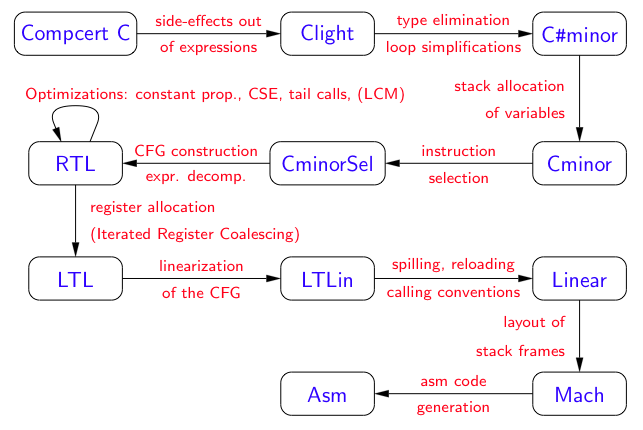
\includegraphics[scale=1]{img/passes.png}
\caption{Verified CompCert passes\hspace{\linewidth}S \textbf{Source: }\texttt{http://compcert.inria.fr/compcert-C.html}}
\label{fig:compcertpasses}
\end{center}
\end{figure}

The compiler used in this work is CompCert~\cite{compcertmanual}.
It supports most of the ISO-C-99 Standard.
It can generate PowerPC, ARM and x86 assembly code.
Because formal program verification is often done at source level, CompCert is a promising tool for the development of critical software~\cite{bedinfranca:hal-00653367}.

Between the source code and the target assembly code, CompCert goes through 25 passes, including several changes of language, all of which using the same memory model.
The first three parse and convert the source code to CompCert C, and the last three perform printing of the assembly code, assembling and linking.
In the middle, 19 back-end passes perform various transformations, 8 of which are optimizations.

\subsubsection{Correctness}
The parser and most of the back-end passes (see \textbf{Fig.\ref{fig:compcertpasses}.}) are verified with Coq.
In CompCert, the behavior of a program is a trace (a list of I/O operations) and an indication on the program's termination.
The correctness theorem of CompCert states that the behavior of the generated code is one of the possible behaviors of the source code (C is non-deterministic). To prove it, it uses a backward simulation (see section~\ref{sec:mixedsim}).

\subsubsection{Optimizations}
CompCert performs the following optimizations:
Instruction selection, Common sub-expression elimination, Tail call elimination, Dead code elimination, Function inlining, Branch tuneling, Constant propagation and Register allocation~\cite{compcertoverview}.
\todo{Examples for the ones that will be used: DCE, DAE, CP, in appendix}
 

\subsection{Memory Models}
\label{subsec:models}
In this section, we present the logical and concrete models with their limits, which motivates the introduction of the quasi-concrete model that has been implemented in this work.

In C semantics, the memory is divided in several \textit{memory blocks}, that contain several memory addresses. Memory blocks can be allocated (through the \texttt{malloc} function for instance), loaded, freed\dots A memory block can contain the values of several variables. 
\subsubsection{Logical Model}
The logical model described here is similar to the one used in~\cite{DBLP:conf/pldi/KangHMGZV15}. However, it slightly differs from CompCert's current logical model described in~\cite{leroy:hal-00703441} (see section~\ref{sec:memupdate}).
In this model, blocks are all logical, meaning that they are not mapped to a physical memory address.
Blocks are a fixed-size array of values.
A validity flag $v$ indicates if the block has been freed.
Pointers are a pair $(l,i)$ of a block identifier and an offset inside that block.
The set $\texttt{Block}$ of blocks is defined with:
$$\texttt{Block}=\{(v,n,c)~|~v\in\texttt{Bool},n\in\mathbb{N},c\in\texttt{Val}^{n}\}$$

With a logical model, programs have infinite memory.
Moreover, a logical model can allow functions to have exclusive control over a logical block.
When a block identifier does not escape when calling a function (\textit{i.e.} if the block identifier cannot be found inside the global variables or the function arguments), then the called function cannot access the block (see section~\ref{sec:memupdate}).% too long sentence?
This allow for many optimizations (see Figure~\ref{fig:examples}).

However, logical models do not support integer-pointer casts. They can allow some arithmetic operations on offsets, but it is impossible to get a physical address from a block.

\subsubsection{Concrete Model}
The concrete model aims to reflect the memory of a real machine, to give a more intuitive semantics to pointer manipulation. 
The memory itself is a $2^{32}$-sized array of values, and \texttt{Allocated}, a list of allocated blocks.
Blocks are simply a pair of a concrete address and a size.
$$\texttt{Block}=\{(p,n)~|~p\in\texttt{int32},n\in\texttt{int32}\}$$
The concrete memory should require from the allocated blocks to be consistent:
$$\textit{No overflow:}\quad\forall (p,n)\in\texttt{Allocated}, [p,p+n]\subseteq]0,2^{32}[$$
$$\textit{No overlap:}\quad\forall (p_1,n_1), (p_2,n_2)\in\texttt{Allocated}, [p_1,p_1+n_1]\text{ and }[p_2,p_2+n_2]\text{ are disjoint.}$$
In the concrete model, integer-pointer cast is possible because concrete addresses are already integer values.

However, optimizations such as constant propagation and dead allocation elimination are not supported in many cases, because external functions might change the value of any address. In the concrete model, there is no ownership of memory blocks, and every address is always accessible.
\subsubsection{Quasi-concrete model}
In~\cite{DBLP:conf/pldi/KangHMGZV15}, a new memory model is presented. The motivation is to have a memory model which allows integer-pointer casting, but still supports common optimizations.
This is achieved with the following definitions.
A block can be either logical or concrete, in which case it has a concrete address. This is represented by the value $p$.
$$\texttt{Block}=\{(v,p,n,c)~|~v\in\texttt{Bool},n\in\mathbb{N},c\in\texttt{Val}^{n},p\in\texttt{int32}\cup\{\undef\}\}$$
The concrete blocks need to be consistent:
$$\textit{No overflow:}\quad\forall (v,p,n,c)\in\texttt{Blocks}, (p\neq\undef~\wedge~ v=\textit{true})\implies[p,p+n]~\subseteq~]0,2^{32}[$$
$$\textit{No overlap:}\quad\forall (p_1,n_1), (p_2,n_2)\in\texttt{Blocks}, (p_1\neq\undef~\wedge~p_2\neq\undef ~\wedge~ v_1=v_2=\textit{true})\implies$$ $$[p_1,p_1+n_1]\text{ and }[p_2,p_2+n_2]\text{ are disjoint.}$$
A pointer is a pair $(l,i)$ of a block identifier and an offset inside that block. If the block $l$ starts at the address $p\neq\undef$, then $(l,i)$ can be cast as the integer $p+i$ and vice versa (thanks to the property of no overlapping, an integer can correspond to at most one valid concrete block).

Optimizations are still be possible with logical blocks, because they do not have concrete addresses, and integer-pointer casts are possible with concrete blocks.
To allow as many optimizations as possible, we should use as many logical blocks as possible. Thus, new blocks should be made logical when allocated.

\subsubsection{The capture function}
However, for each pointer to integer cast, we need a concrete block. Then we transform each pointer to integer cast by adding a \textit{capture} function just before it. This function transforms a logical block into a concrete one, giving it a concrete address that still satisfies the memory consistency. Its semantics are described section~\ref{sec:capturesem}.
It introduces non-determinism in every language of CompCert (including the assembly), because a block can be captured at several addresses. This is handled in section~\ref{sec:mixedsim}.

The quasi-concrete is described in many details in~\cite{DBLP:conf/pldi/KangHMGZV15}.
\subsubsection{Optimization and casts examples}

\lstset{}
\begin{figure}
\begin{subfigure}{.33\textwidth}
  \begin{lstlisting}
  extern void g();
  int f(void) {
    int a = 0;
    
    g();
    return a;
  }
  \end{lstlisting}
  \caption{Logical block example}
  \label{fig:logical}
\end{subfigure}%
\begin{subfigure}{.33\textwidth}
  \begin{lstlisting}
  extern void g();
  int f(void) {

    
    g();
    return 0;
  }
  \end{lstlisting}
  \caption{After CP and DAE}
  \label{fig:cpdae}
\end{subfigure}
\begin{subfigure}{.33\textwidth}
  \begin{lstlisting}
  extern void g();
  int f(void) {
    int a = 0;
    int p = (int) &a;
    g();
    return a+p;
  }
  \end{lstlisting}
  \caption{Concrete block example}
  \label{fig:concrete}
\end{subfigure}
\caption{Examples of optimizations and casts}
\label{fig:examples}
\end{figure}

% first example
Consider the program Fig.\ref{fig:logical}. Using a logical memory model, Constant Propagation is allowed, because no pointer to the block of \texttt{a} is available from \texttt{g()}, and thus the external call cannot change the value of \texttt{a}. Then, the compiler can replace \texttt{return a;} with \texttt{return 0;}. After that, Dead Allocation Elimination can remove the allocation of \texttt{a}, now unused. The optimized program can be seen Fig.\ref{fig:cpdae}.
Using a concrete model, the block containing the value of \texttt{a} is mapped to a concrete address. Without more information on \texttt{g()}, it should be assumed that it might change the value of \texttt{a}. Thus, the program cannot be optimized.
Using the quasi-concrete model, a new block is allocated for the allocation of \texttt{a}. Since it is new, it is a logical block, without a concrete address. Thus, \texttt{g()} cannot modify the value of \texttt{a} and the program can once again be transformed into Fig.\ref{fig:cpdae}.

%second example
Consider the program Fig.\ref{fig:concrete}, where the address of \texttt{a} is cast as an integer. Unlike with a concrete model, using a logical model defines no semantics for this program. With the quasi-concrete model, the block containing the value of \texttt{a} is transformed into a concrete one just before the cast. No optimization is possible, because \texttt{g()} can possibly modify any concrete block, but the semantics of the program is defined.




\section{Related Works}
% problems with UB
It has been established that writing programs with undefined behavior can lead to difficult-to-find bugs.
For instance, some compilers can optimize code with the assumption that the program never encounters undefined behavior. This can result in produced code that does not behave as expected by the programmers~\cite{DBLP:conf/apsys/WangCCJZK12}.

% identify UB-unstable code
A first solution to this issue is to identify the code whose optimization is based on undefined behaviors, as presented in~\cite{DBLP:conf/sosp/WangZKS13}.

% refine semantics
However, a more common approach is to extend the semantics expressiveness of the C language, ruling out undefined behaviors.
Many works have revolved around giving a formal semantics to the C language refining the informal semantics of the ISO standard.
This is what~\cite{DBLP:conf/pldi/KangHMGZV15} and this paper aim to achieve by refining the C semantics for pointer manipulation.

% Symbolic values
For the same purposes, some have investigated the use of a concrete memory model for C semantics~\cite{DBLP:conf/popl/TuchKN07}\cite{Norrish98cformalised}.
More recently,~\cite{besson:hal-01093312} and~\cite{DBLP:conf/itp/BessonBW15} present the use of a new memory model using symbolic values. The idea is to use symbolic values instead of expressions to delay their evaluation. This successfully gives semantics to several C idioms: alignment constraints, bit-fields\dots However, as it is a deterministic semantics, programs that introduce non-deterministic behaviors due to allocation are still undefined.

% back to our work
In this work, we present a new approach to deal with non-determinism in CompCert, and give semantics to every integer-pointer casts and pointer manipulation.

%Other related works
Another approach to deal with finite memories has been used in CompCertTSO~\cite{DBLP:journals/jacm/SevcikVNJS13}, where all memory operations are done on a single finite logical block. Even if the memory model not the quasi-concrete model, the authors of~\cite{DBLP:conf/pldi/KangHMGZV15} are confident that the quasi-concrete model could handle address threads like CompCertTSO.
The quasi-concrete model could also be used with other works of semantics extension, such as the union types and strict aliasing of~\cite{DBLP:conf/cpp/Krebbers13} or the universal pointer type of~\cite{DBLP:conf/itp/KrebbersLW14}.


\section{Contribution}
The goal of this work is to implement the quasi-concrete model in CompCert.
In a first part, we show how the definitions have been modified to fit into CompCert.
In a second part, we show how the definition of memory injection has to be modified. It changes a lot of proofs in CompCert. As a consquence, we have to change the way CompCert performs abstract analysis.
In a third part, we present how adding non-determinism in every language of CompCert prevents us from using the same correctness proofs. We design a new proof, using mixed simulations. It relies on the observation that non-deterministic behavior is only encountered when using the capture function.
Finally, we define and implement semantics for integer-pointer casts. This heavily relies on the semantics of the new capture function, meant to turn logical blocks into concrete blocks when needed.


\section{Evaluation}
\label{sec:eval}
\begin{figure}[H]
\begin{subfigure}{.48\textwidth}
  \begin{lstlisting}[language=C,basicstyle=\small]
extern void g();
int f() {
  int a = 0;
  int* q = &a;
  g();
  return a; }
\end{lstlisting}
\end{subfigure}
\begin{subfigure}{.48\textwidth}
  \begin{lstlisting}[basicstyle=\small]
f() {
    6:	x4 = 0
    5:	int32[stack(0)] = x4
    4:	nop
    3:	x3 = "g"()
    2:	x2 = 0
    1:	return x2 }
\end{lstlisting}
\end{subfigure}
\caption{Constant propagation on logical blocks}
\label{fig:cplogical}
\end{figure}
\begin{figure}[H]
\begin{subfigure}{.48\textwidth}
  \begin{lstlisting}[language=C,basicstyle=\small]
extern void g();
int f() {
  int a = 0;
  int* q = &a;
  int b = (int) q;
  g();
  return a; }
\end{lstlisting}
\end{subfigure}
\begin{subfigure}{.48\textwidth}
  \begin{lstlisting}[basicstyle=\small]
f() {
    8:	x5 = 0
    7:	int32[stack(0)] = x5
    6:	x2 = stack(0) (int)
    5:	_ = builtin __capture(x2)
    4:	nop
    3:	x4 = "g"()
    2:	x3 = int32[stack(0)]
    1:	return x3 }
\end{lstlisting}
\end{subfigure}
\caption{No Constant propagation on concrete blocks}
\label{fig:cpconcrete}
\end{figure}

The correctness of CompCert with the new memory model hasn't been entirely proved yet.
The remaining proofs are most of the proofs of mixed simulations.
However, we remain confident that such a mixed simulation exists for every pass. One mixed simulation has been proved (\texttt{CSEproof}, an optimization pass), and others should be very similar. The intuition behind any mixed simulation proof is the same: use the previous forward simulation proof to prove a local forward simulation of non-external states, then use the new properties of external calls to prove the local backward simulation of external states.

Even if the semantics of casting has not been fully implemented yet, it is already possible to compile some C programs with our modified version of CompCert. We can see that the new model successfully gives semantics to integer-pointer casting, but also allow optimizations when using logical blocks.
This is illustrated Figure~\ref{fig:cplogical}. We can see that constant propagation is done, and the program returns 0. This is explained by the fact that the memory block of \texttt{a} is logical, and thus the function \texttt{f()} has ownership of this memory block. The compiler deduces that \texttt{a} cannot be accessed by the function \texttt{g()}, and thus performs constant propagation.
However, if the block is made concrete, then \texttt{f()} looses ownership of \texttt{a} and constant propagation should not be done. This is illustrated Figure~\ref{fig:cpconcrete}, where the memory block of \texttt{a} has to be captured due to the pointer-to-integer cast.


\section{Conclusion}
\begin{frame}{\secname}

  \begin{exampleblock}{Results}
    \begin{itemize}
    \item The new memory model has been implemented in CompCert.
    \item It successfully gives semantics to Integer-Pointer casts.
    \item It allows optimizations.
    \item The proof of correctness is almost finished.
    \end{itemize}
  \end{exampleblock}
  \vfill
  \begin{block}{Future Work}
    \begin{itemize}
    \item Finish the mixed simulations proofs.
    \item Finish implementation of the integer-pointer cast semantics.
    \end{itemize}
  \end{block}
  
\end{frame}


\begin{frame}{}
  %last takeaway frame
  \begin{center}
  \begin{figure}
  \begin{tikzpicture}[%
      every node/.style={rectangle, font=\tiny},
      shorten >=2pt,
      node distance=1.1cm
    ]
    \node (cc) [] {CompCert C};
    \node (cstrat) [right=of cc] {CStrategy};
    \node (clight) [right=of cstrat] {Clight};
    \node (dots) [right=of clight] {\dots\vphantom{C}};
    \node (mach) [right=of dots] {Mach};
    \node (asm) [right=of mach] {ASM};
    \node (atcstrat) [below=of cstrat] {\at{CStrategy}};
    \node (atclight) [below=of clight] {\at{Clight}};
    \node (atdots) [below=of dots] {\at{\dots}};
    \node (atmach) [below=of mach] {\at{Mach}};
    \path [draw] (cc) edge[<-, above] node {1. backward} (cstrat);
    \path [draw] (cstrat) edge[<->, above] node {1. mixed} (clight);
    \path [draw] (clight) edge[<->, above] node {1. mixed} (dots);
    \path [draw] (dots) edge[<->, above] node {1. mixed} (mach);
    \path [draw] (mach) edge[<->, above] node {1. mixed} (asm);
    \path [draw] (atcstrat) edge[<-,below right] node {2. backward} (clight);
    \path [draw] (atclight) edge[<-,below right] node {2. backward} (dots);
    \path [draw] (atdots) edge[<-,below right] node {2. backward} (mach);
    \path [draw] (atmach) edge[<-,above left] node {2. backward} (asm);
    \path [draw] (cc) edge[<-,above right] node {3. backward} (atcstrat);
    \path [draw] (atcstrat.300) edge[<-, bend right=90, below] node {3. backward} (atclight);
    \path [draw] (atclight.300) edge[<-, bend right=90, below] node {3. backward} (atdots);
    \path [draw] (atdots.300) edge[<-, bend right = 90, below] node {3. backward} (atmach);
    \path [draw] (cc) edge[<-, bend right=90, below] node {4. backward} (asm);
  \end{tikzpicture}
  \end{figure}
  \end{center}
\end{frame}


%
% ---- Bibliography ----
%
\newpage
\nocite{*}
\bibliographystyle{plain}
\bibliography{../bib/intptrcast.bib}

\end{document}
